\vsssub
\subsubsection{~Unresolved obstacles} \label{sub:num_obst}
\conthead{\ws}{H. L. Tolman}

\noindent
Even at the time of the original tuning of \ws\ version 1.15
\citep{tol:OMB02a}, it was clear that unresolved islands groups are a major
source of local wave model errors. This was illustrated in some more detail in
\citet[][Fig.~3]{tol:Waves01a}, and \citet[][Fig.~8]{tol:WaF02}. In \ws, a
methodology from \swan\ \citep{art:BRH99,man:SWAN3} was adopted to apply the
effects of unresolved obstacles at the cell boundaries of the spatial grid
within the numerical scheme. In this approach, the numerical fluxes between
cells through their common boundary are suppressed according to the degree of
obstruction provided by the unresolved obstacle. In this approach, the
numerical propagation scheme of the \uq\ scheme of Eq.~(\ref{eq:uq_xy_tot}) is
modified as

% eq:uq_xy_obstr

\begin{equation}
\cN_{i,j,l,m}^{n+1} = \cN_{i,j,l,m}^n +
\frac{\Delta t}{\Delta \phi} \left [ \alpha_{i,-} \cF_{i,-} - \alpha_{i,+} \cF_{i,+} \right ]
\: , \label{eq:uq_xy_obstr} \end{equation}

\begin{figure} \begin{center}
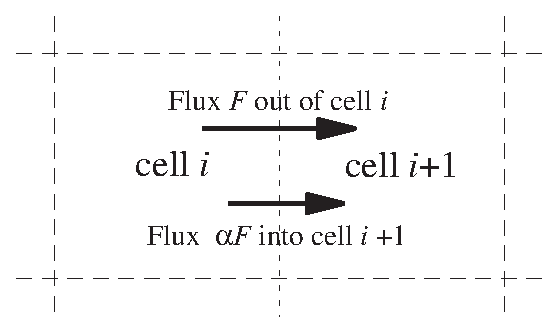
\epsfig{file=./num/obstr.eps,angle=0,width=2.2in}
\caption{Treatment of unresolved obstacles. Common cell
         boundary (dotted line) has transparency $\alpha$. Dashed lines
         represent other cell boundaries. Numerical flux from left to right.}
         \label{fig:obstr} \botline
\end{center}
\end{figure}

\noindent
where $\alpha_{i,-}$ and $\alpha_{i,+}$ are `transmissions' of the
corresponding cell boundaries, ranging from 0 (closed boundary) to 1 (no
obstructions). For outflow boundaries, transparencies by definition are 1,
otherwise energy will artificially accumulate in cells. For inflow boundaries,
transparencies less than 1 result in elimination of obstructed energy at the
cell boundary. This approach is illustrated in
Fig.~\ref{fig:obstr}. Note that a similar approach is easily adopted in the
first- and second-order schemes.  Note, furthermore, that an alternate
obstruction approach with obstructions as a function of the spectral direction
$\theta$ has been used by \cite{art:HY96} and \cite{art:HMM00}.

Two methods for defining the obstructions are available in the model. The
first defines the obstructions directly at the grid boundary. This requires
the generation of staggered depth-transparency grids. The second allows the
user to define depths and transparencies at the same grid. In this case, the
transparency at the inflow boundary becomes $0.5(1+\alpha_i)$, and the outflow
transparency by definition is 1. To complete the total transparency
$\alpha_i$, the next cell in the flow direction will have an inflow
transparency $2\alpha_i/(1+\alpha_i)$. If consecutive cells are partially
obstructed, the product of individual transparencies is applied.

This approach can also be used to continuously model the effects of ice
coverage on wave propagation. This is discussed in \para\ref{sub:num_ice}.
Details of the sub-grid treatment of islands and ice can be found in
\cite{tol:OMOD03a}. A study of impacts of this approach in large-scale wave
models is presented in \cite{tol:OMB02b,tol:OMOD03a}.

The default setting of \ws\ is to not include sub-grid modeling of
obstacles. Generating obstruction grids can be labor intensive. For this
reason, an automated approach for generating bottom and obstruction grids was
developed by \cite{tol:MMAB07a, tol:OMOD08a}.  Note that this option does not
involve compile-level choices, but is entirely controlled from the grid
preprocessor (see Chapter \ref{chapt:run}).

